\chapter{Results and Discussion}
\label{chap:evaluation}

As a result of the ETL-Application a database with structured information about the national council is available now and can be used for further purposes. This database has been used for analysis and the results got visualized via a web application which is accessible for everybody. Figure \ref{fig:start_page_prototype} shows the start page of this application. Furthermore, the relation graphs of several periods get discussed in the sections \ref{sec:relations_clubs} and \ref{sec:relations_pol}. 

\begin{figure}[h]
	\center
	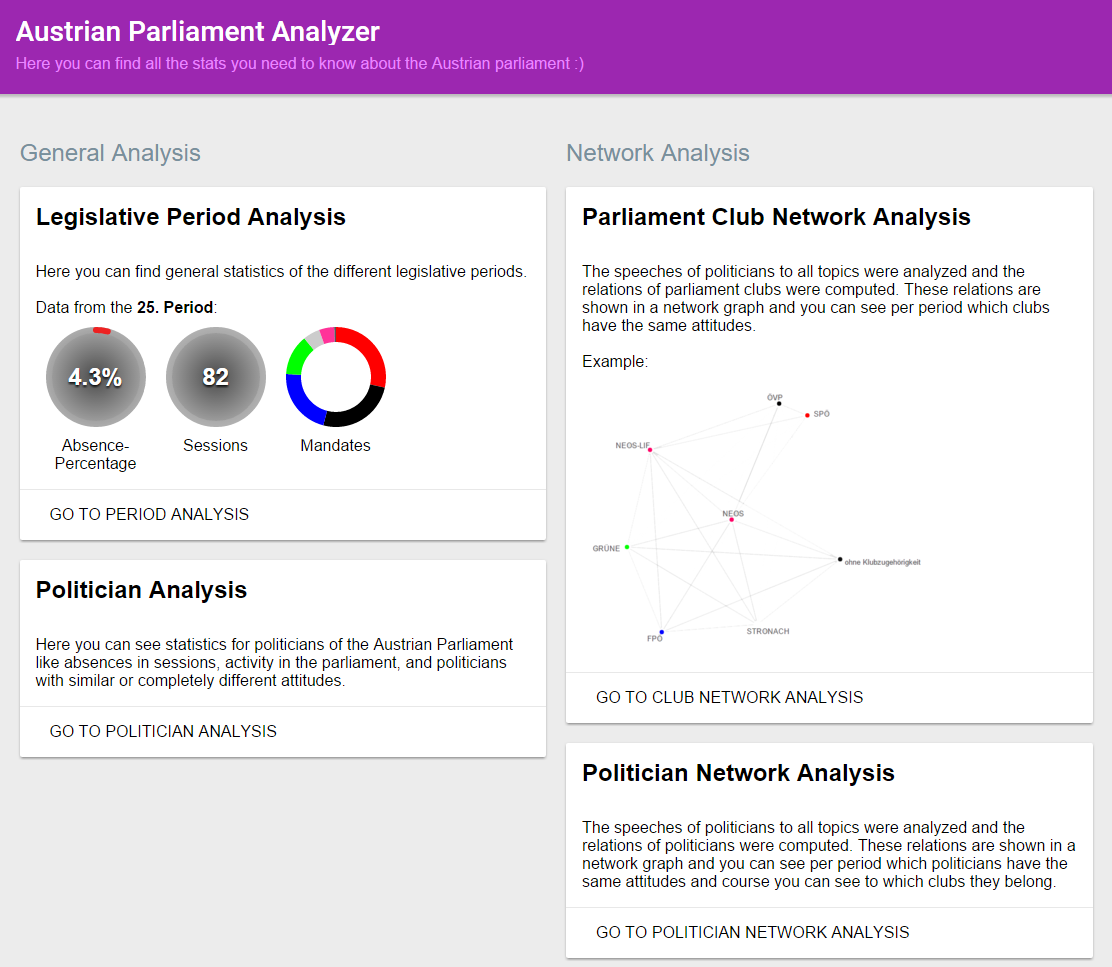
\includegraphics[width=0.75\textwidth]{imgs/result_start_page}
	\caption{Start Page of the Prototype Web Application}
	\label{fig:start_page_prototype}
\end{figure}

\section{Relations of Parliament Clubs}
\label{sec:relations_clubs}
Figure \ref{fig:club_graphs1} shows the created relation graphs of the parliamentary clubs of the 25. and 22. legislative periods. The graphs visualize the relations among the clubs through the distance of the nodes. The more positive the relation between two clubs is, the closer they appear together in the graph and the thicker is the edge between them. Only positive edges are shown in the graph, as the graph would look too confusing and messy if the negative edges were also shown. In all graphs shown, one can easily see that there are always two main groups of parliamentary clubs visible in the parliament: Those which are in government and those which are in opposition. In table \ref{table:gov_opp_parties} the parties are listed per period weather they were in government or in opposition. 
In the current period (25.) you can see that the governing parties (ÖVP and SPÖ) have a strong positive relationship and that there are only minor positive relationships between the governing parties and the NEOS party. All other parties in the opposition have negative relationships to the government.

\begin{figure}
%\begin{tabular}{ c  c }
%	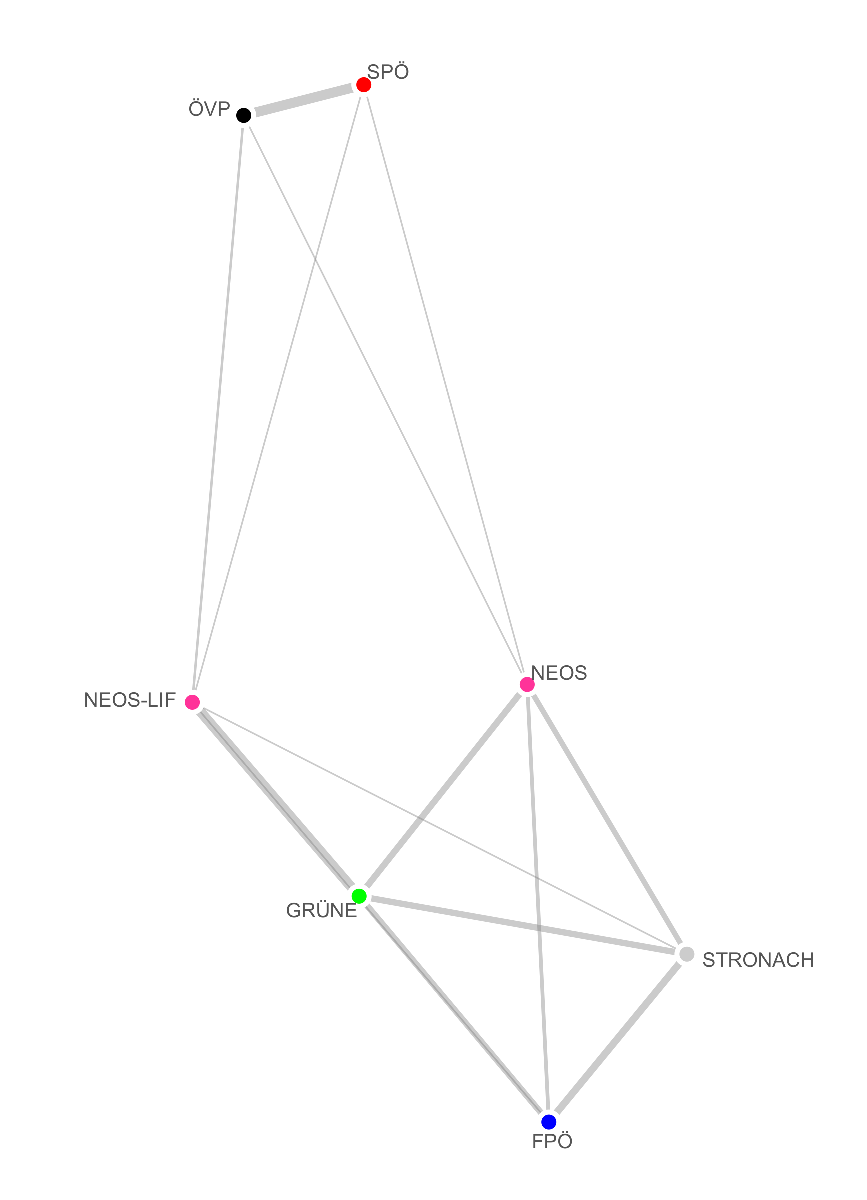
\includegraphics[width=0.47\textwidth]{imgs/graphs/club-graphs/graph_25.eps} 
	%& 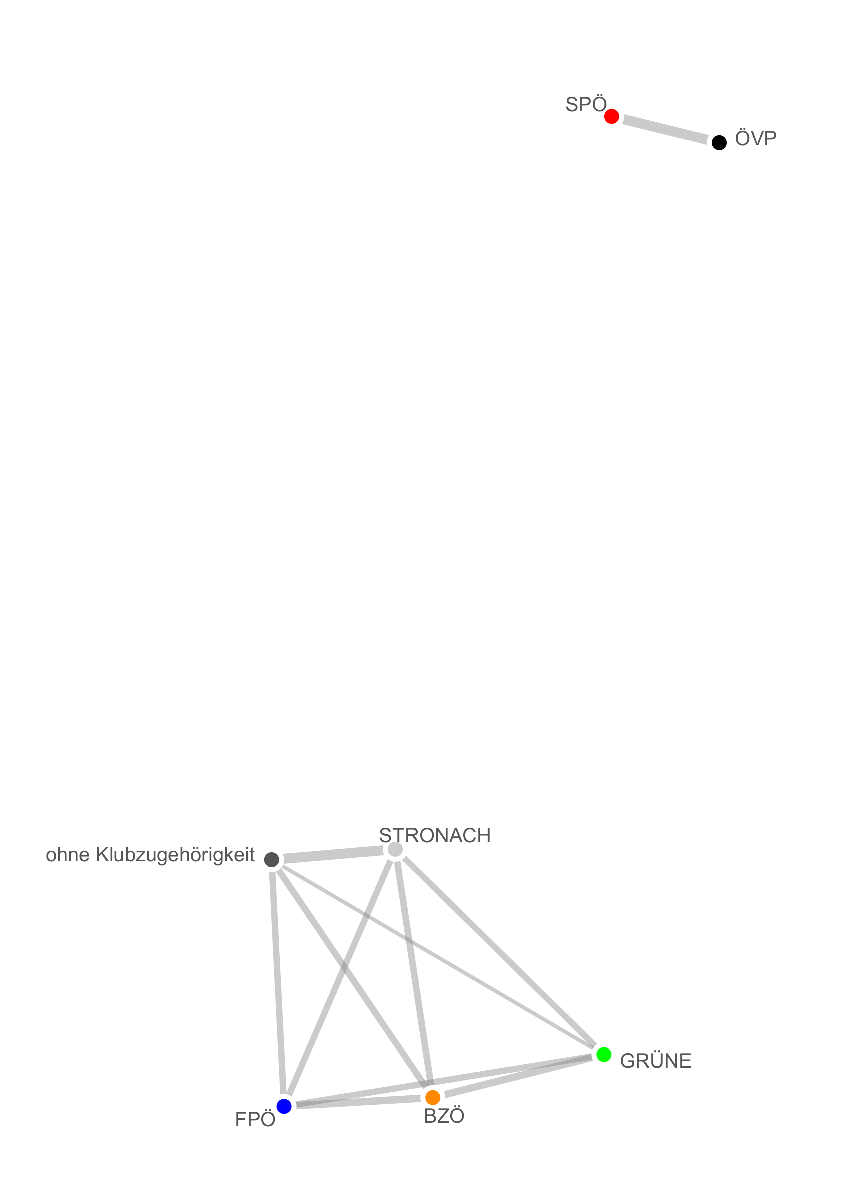
\includegraphics[width=0.3\textwidth]{imgs/graphs/club-graphs/graph_24.eps} 
%	& 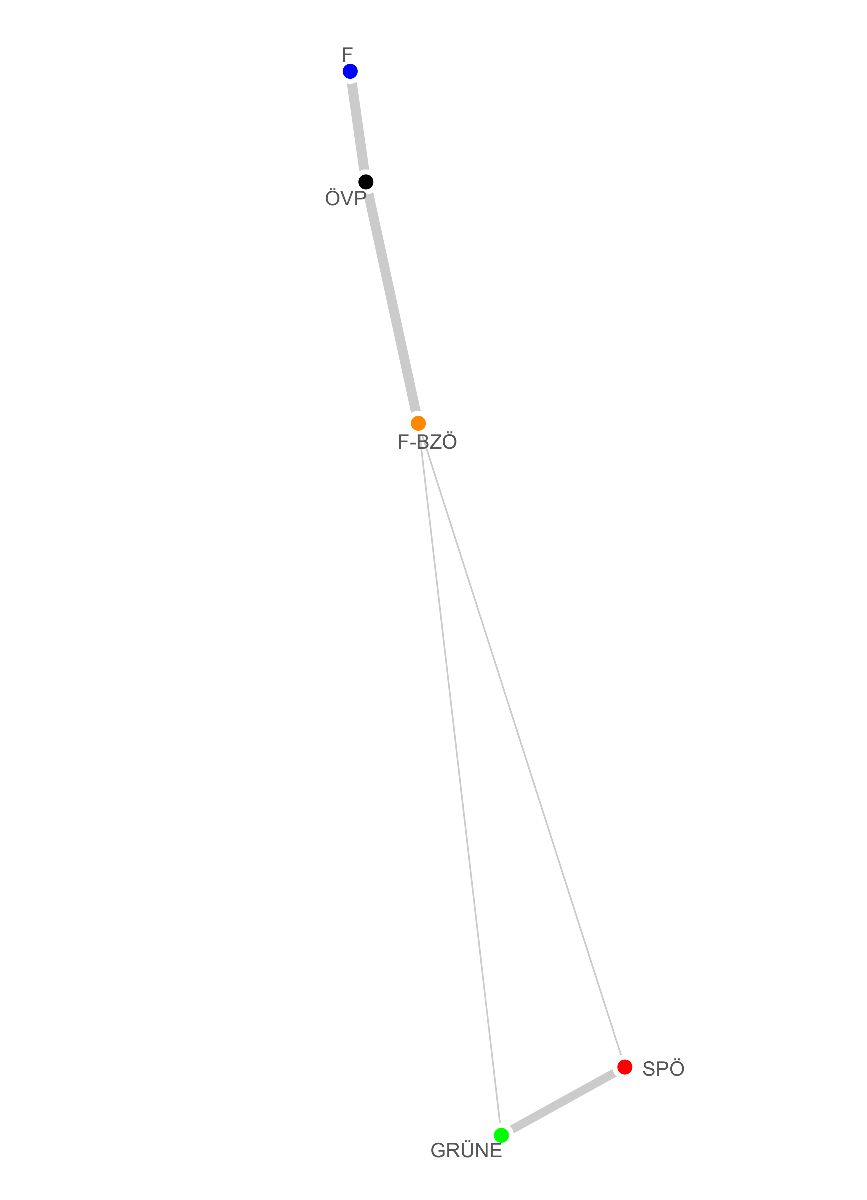
\includegraphics[width=0.47\textwidth]{imgs/graphs/club-graphs/graph_22.eps}
%	\\
%	(a) 25. Period 
	%& (b) 24. Period 
%	& (c) 22.Period
%\end{tabular}
	\center
	\begin{tabular}{ c }
		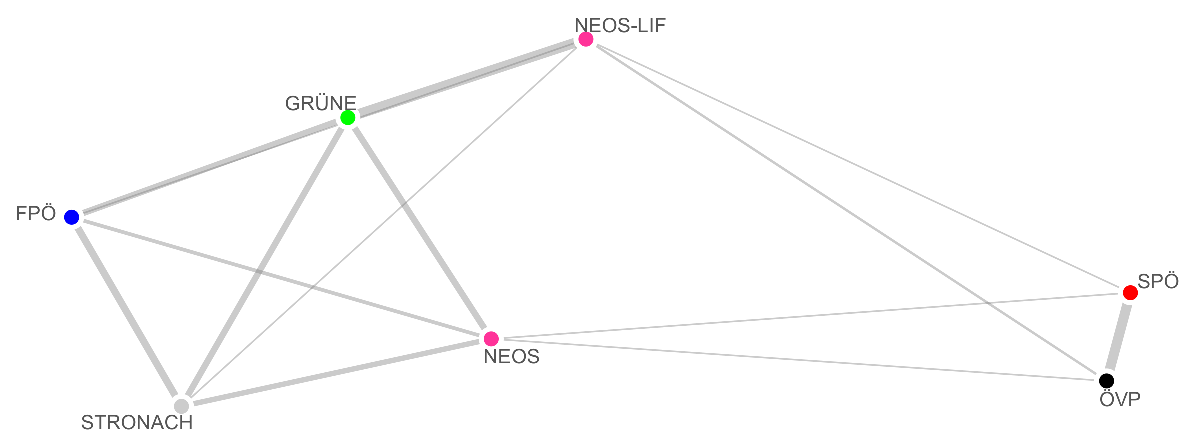
\includegraphics[width=0.49\textwidth]{imgs/graphs/club-graphs/horizontal/graph_25.eps}
		\\
		(a) 25. period - on $25^{th}$ of December, 2015
		\\
		\\
		\hline
		\\
		\\
		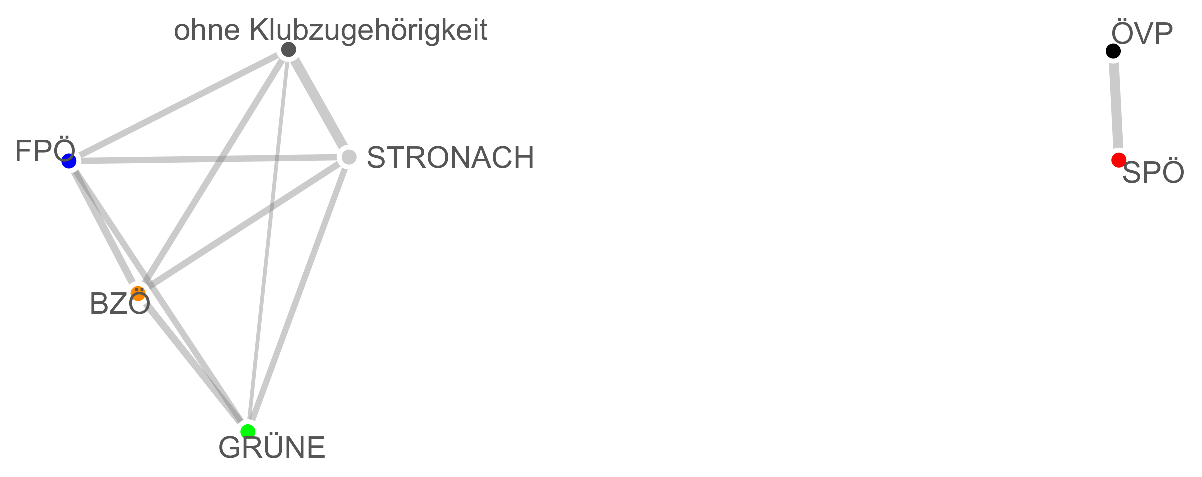
\includegraphics[width=0.7\textwidth]{imgs/graphs/club-graphs/horizontal/graph_24.eps}
		\\
		(b) 24. period
		\\
		\\
		\hline
		\\
		\\
		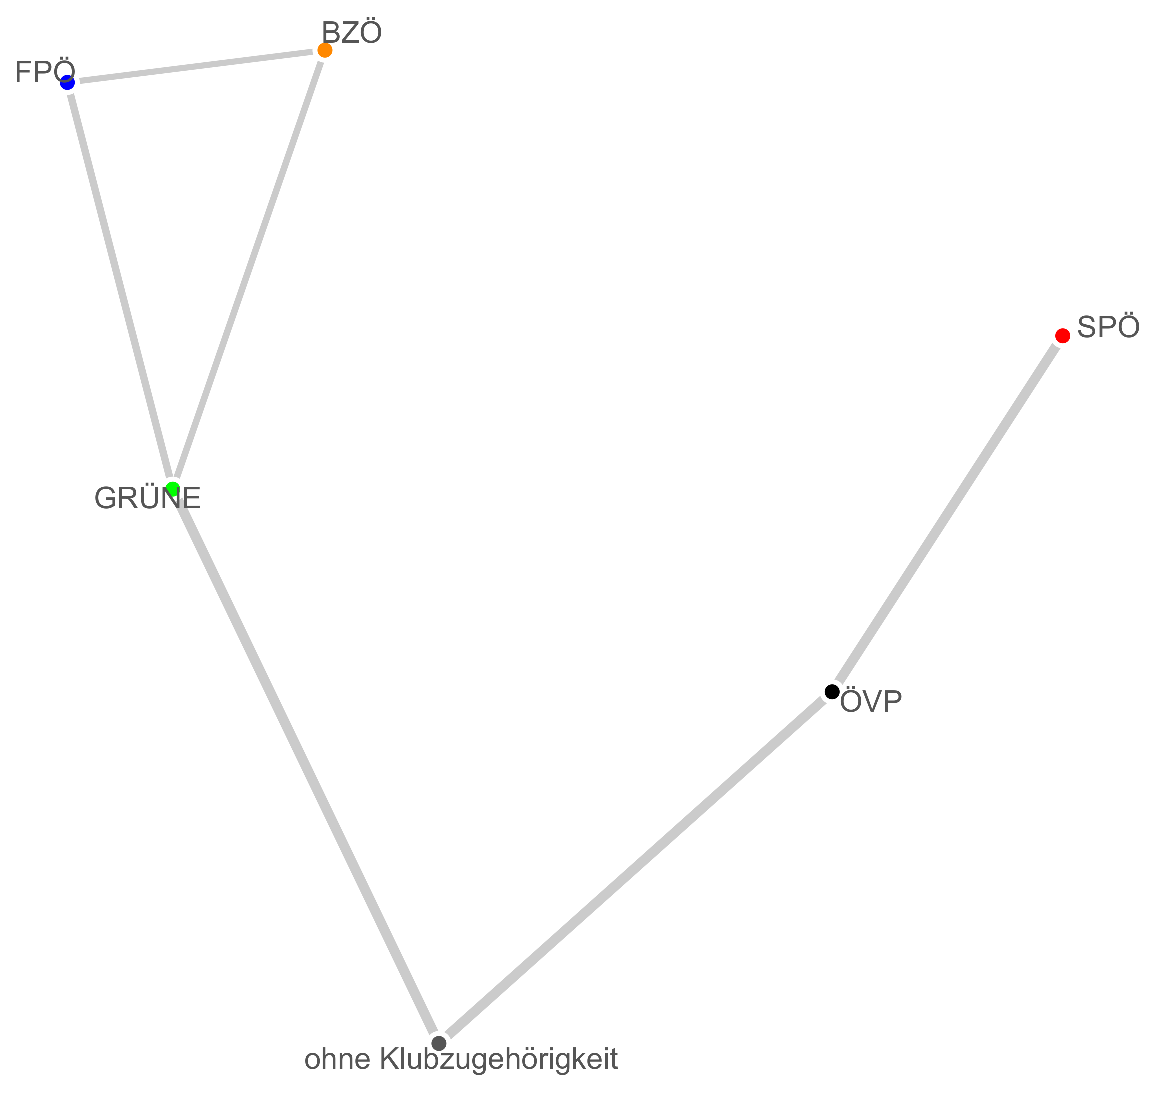
\includegraphics[width=0.55\textwidth]{imgs/graphs/club-graphs/horizontal/graph_23.eps}
		\\
		(c) 23. period
		%\\
		%\\
		%\\
		%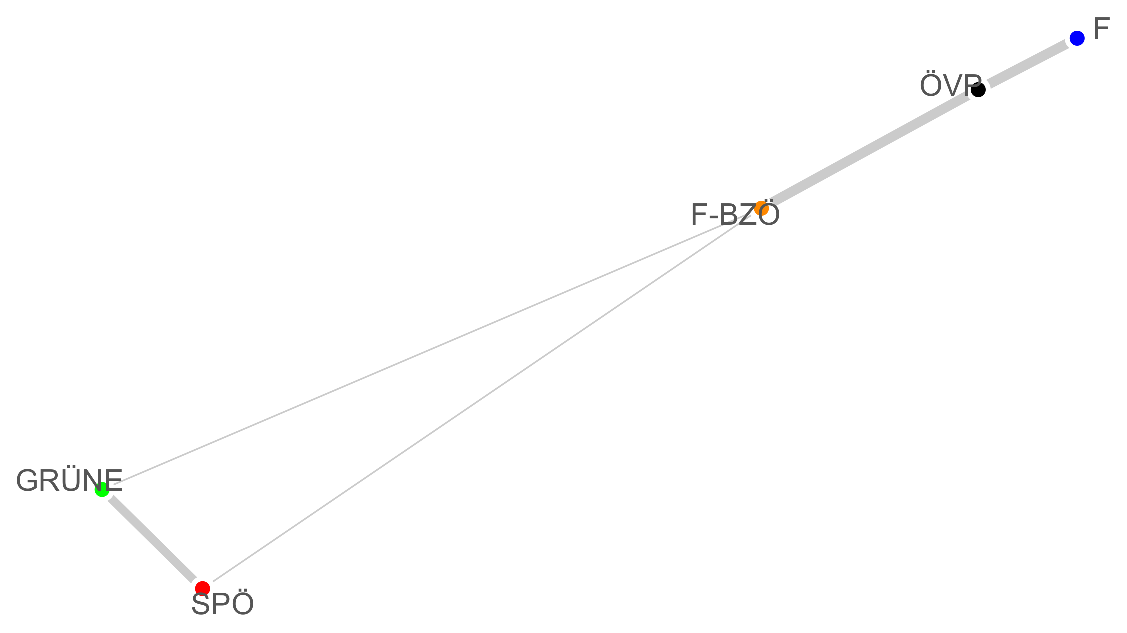
\includegraphics[width=0.6\textwidth]{imgs/graphs/club-graphs/horizontal/graph_22.eps}
		%\\
		%(c) 22. period
		
	\end{tabular}
	

	\caption{Club Relation Graphs}
	\label{fig:club_graphs1}
\end{figure}

\begin{table}[h]

\centering
\bgroup
\def\arraystretch{1.2}
\begin{tabular}{| p{4cm} | p{3cm} | l |}
\hline
  Legislative Period & Governing Parties & Opposition  \\
\hline
\hline
  20. Period: 1995 - 1999 & SPÖ, ÖVP & FPÖ, Grüne, Liberale \\
\hline
  21. Period: 1999 - 2002 & ÖVP, FPÖ & SPÖ, Grüne \\
\hline
  22. Period: 2002 - 2006 & ÖVP, FPÖ, BZÖ\footnote{The BZÖ was in government from $17^{th}$ of April, 2005} & SPÖ, Grüne \\
\hline
  23. Period: 2006 - 2008 & SPÖ, ÖVP & FPÖ, Grüne, BZÖ \\
\hline
  24. Period: 2008 - 2013 & SPÖ, ÖVP & FPÖ, Grüne, Stronach, BZÖ \\
\hline
  25. Period: since 2013 & SPÖ, ÖVP & FPÖ, Grüne, NEOS, Stronach \\
\hline

\end{tabular}
\egroup
\caption{Government and Opposition in the Legislative Periods 20 to 25}
\label{table:gov_opp_parties}
\end{table}


\section{Relations of Politicians}
\label{sec:relations_pol}
Similar graphs to the ones in section \ref{sec:relations_clubs} were created for politicians. Figure ... shows this graphs for the legislative periods ... 

\section{Government - Opposition Relation}
\label{sec:gov_opp_relation}
Table \ref{table:gov_opp_relation} shows the results of the measures taken for the government-opposition relation, inner government cohesion and inner opposition cohesion. Figure \ref{fig:gov_opp_relation} shows the changes over time of these values. The values show basically that the two main groups in the parliament - the government and opposition - are highly distinct. The government-opposition relation is negative in every discussed period. This means that there is an overall tendency of politicians in government and opposition to have a different opinion. The values differ in the periods, the 20. period shows a the most negative value with $-0.85$. This means that only in $7.5$\% of the speeches a politician in government and opposition had the same opinion on a certain topic, in all other speeches they had contrary ones. In the current period, this inter relationship value is still negative, but it is a lot less negative. The relation coefficient is $-0.374$ which means that in $31.3$\% of the speeches government and opposition have the same opinion.



\begin{table}[h]

\centering
\bgroup
\def\arraystretch{1.2}
\begin{tabular}{| p{2cm} | p{3cm} | p{3cm} | p{3cm} |}
\hline
  Legislative Period & Government-Opposition Relation & Inner-Government Cohesion & Inner-Opposition Cohesion \\
\hline
\hline
  20. Period & $-0.85$ & +1.00 & +0.86 \\
\hline
  21. Period & $-0.695$ & +0.985 & +0.908 \\
\hline
  22. Period & $-0.567$ & +1.00 & +0.938 \\
\hline
  23. Period & $-0.382$ & +0.994 & +0.765\\
\hline
  24. Period & $-0.52$ & +1.00 & +0.768\\
\hline
  25. Period & $-0.374$ & +1.00 & +0.676\\
\hline

\end{tabular}
\egroup
\caption{Government-Opposition Relation, Inner Government- and Inner Opposition Relation for the Legislative Periods 20 to 25}
\label{table:gov_opp_relation}
\end{table}

\begin{figure}
\center
	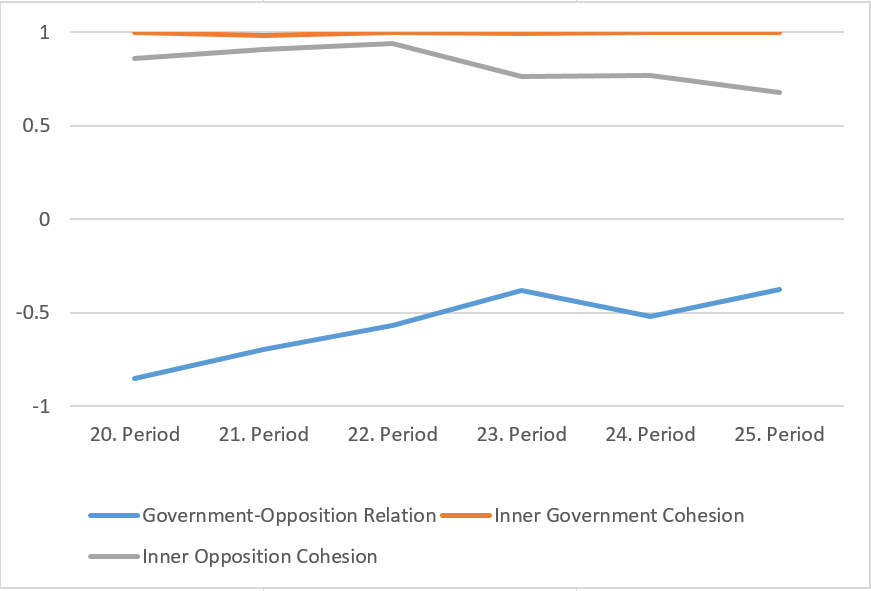
\includegraphics[width=0.75\textwidth]{imgs/gov_opp_rel_graph}
	\caption{Development of the Inter-Government-Opposition Relationship Coefficient and Inner Cohesion Values over Time}
	\label{fig:gov_opp_relation}
\end{figure}